\documentclass[de]{./../../common/SurferDesc}%%%%%%%%%%%%%%%%%%%%%%%%%%%%%%%%%%%%%%%%%%%%%%%%%%%%%%%%%%%%%%%%%%%%%%%
%
% The document starts here:
%
\begin{document}
\footnotesize
% Weltrekordfl�chen

%%% 1.Tafel

%%%%%%%%%%%%%%%%%%%%%%%%%%%%%

\begin{surferPage}
  \begin{surferTitle}Die Cayley-Kubik\end{surferTitle}  \\
  Diese Kubik (Fl�che vom Grad $3$) besitzt 
    gleichzeitig vier doppelkegelf�rmige Singularit�ten. Sie ist nach
    Arthur Cayley benannt, der viel �ber kubische Fl�chen geforscht hat.

    Es war aber Ludwig Schl�fli, der als erster 1863 diese Fl�chen
    systematisch danach untersuchte, welche Typen von Singularit�ten auftreten
    k�nnen.  
    Z.B.\ kann man in seiner Arbeit nachlesen, warum es nicht mehr als $4$
    singul�re Punkte gleichzeitig auf einer kubischen Fl�che geben kann, 
    d.h.\ $\mu(3)=4$. 
    
    Auch Felix Klein untersuchte um 1900 kubische Fl�chen auf ihre
    m�glichen Gestalten; seine Idee war es, diese Frage
    von der Cayley-Kubik ausgehend durch leichte Ver�nderungen zu beantworten:
    Durch Aufweiten, Auftrennen oder Zusammenf�hren von Doppelkegeln konnte er
    tats�chlich alle anderen Gestalten erhalten, z.B.: \newline
    \begin{center}
      \vspace{-0.2cm}
      \begin{tabular}{@{}c@{\ }c@{\ }c@{\ }c@{}}
        \begin{tabular}{@{}c@{}}
          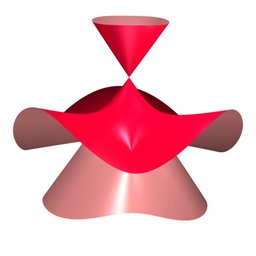
\includegraphics[width=1.35cm]{./../../common/images/cayley_cubic_0}
        \end{tabular}
        &
        \begin{tabular}{@{}c@{}}
          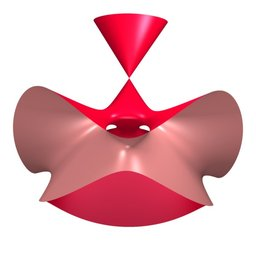
\includegraphics[width=1.35cm]{./../../common/images/cayley_cubic_1}
        \end{tabular}
        &
        \begin{tabular}{@{}c@{}}
          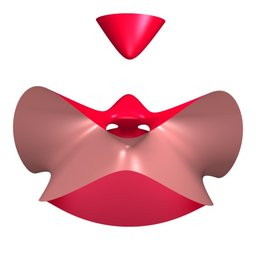
\includegraphics[width=1.35cm]{./../../common/images/cayley_cubic_2}
        \end{tabular}
        &
        \begin{tabular}{@{}c@{}}
          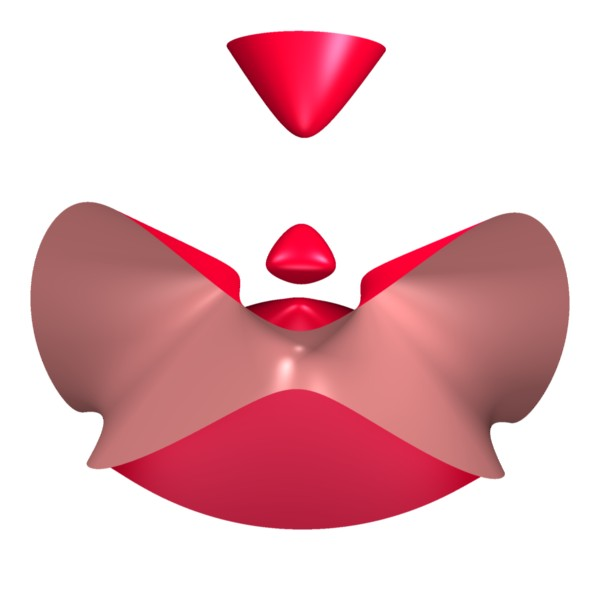
\includegraphics[width=1.35cm]{./../../common/images/cayley_cubic_3}
        \end{tabular}
      \end{tabular}
    \end{center}

  \begin{surferText}
     \end{surferText}
\end{surferPage}

%%%%%%%%%%%%%%%%%%%%%



\end{document}
%
% end of the document.
%
%%%%%%%%%%%%%%%%%%%%%%%%%%%%%%%%%%%%%%%%%%%%%%%%%%%%%%%%%%%%%%%%%%%%%%%
